\section{One website and the engineering behind it}\label{sec:website}

The three apps are built and deployed together as one static site on GitHub Pages \citep{ghpages}. A root script builds the homepage and the three apps into one folder under their paths, and one GitHub Actions workflow publishes it on every push to \code{main}. Every app uses a relative Vite \code{base} (\code{./}), so assets load under any sub-path. Projection Lab runs on Pages in its static data mode (\cref{sec:p1}). Trondheim 3D reads its Cesium ion token from a repository secret, and the production token is restricted to the Pages origin. Each project has its own CI workflow (lint, tests, build): 18 tests for Projection Lab, 54 for Trondheim 3D and 26 for the 3DGS Viewer. After the first deployment, all workflows passed, and a Playwright round trip (homepage, each app, homepage) at 1600 and 390\,px showed no console errors or failed requests (\cref{fig:mobile}).

\begin{figure}[htbp]
\centering
\begin{subfigure}{0.24\textwidth}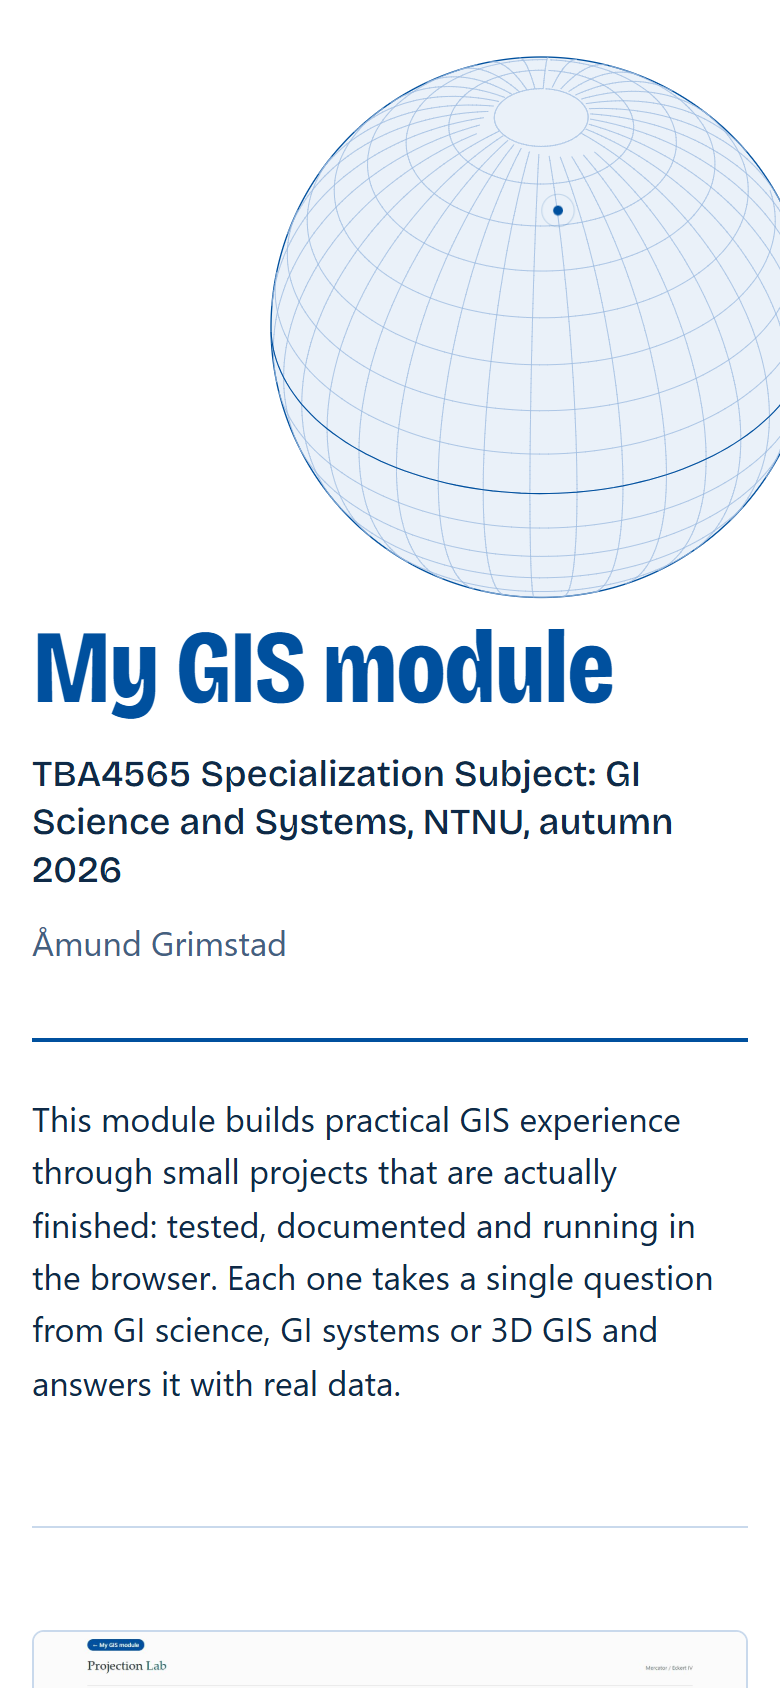
\includegraphics[width=\linewidth]{site-03-homepage-mobile.png}\caption{Homepage}\end{subfigure}\hfill
\begin{subfigure}{0.24\textwidth}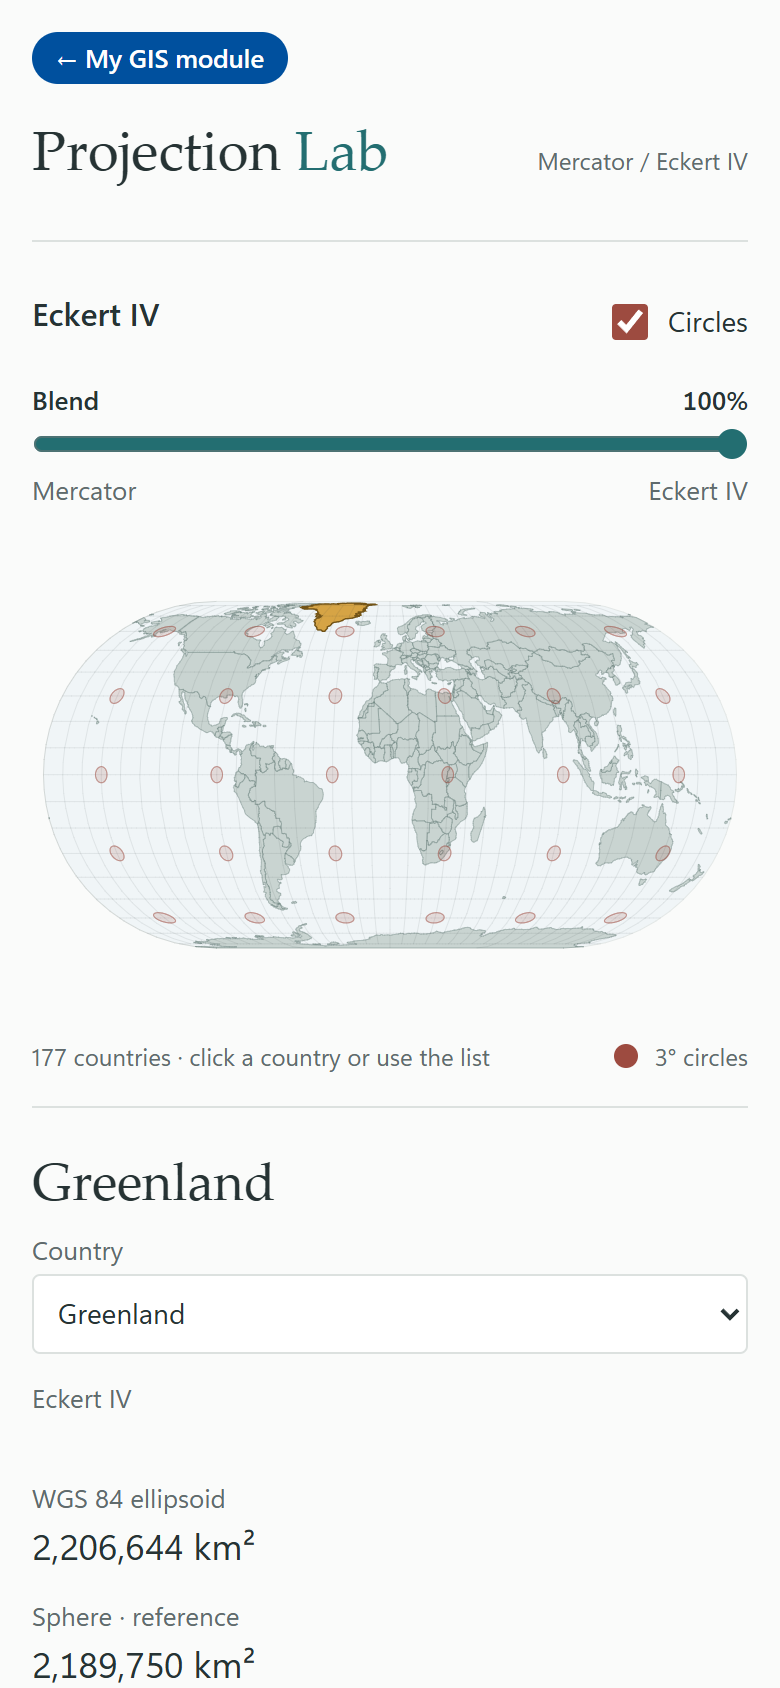
\includegraphics[width=\linewidth]{project-1-06-mobile.png}\caption{Projection Lab}\end{subfigure}\hfill
\begin{subfigure}{0.24\textwidth}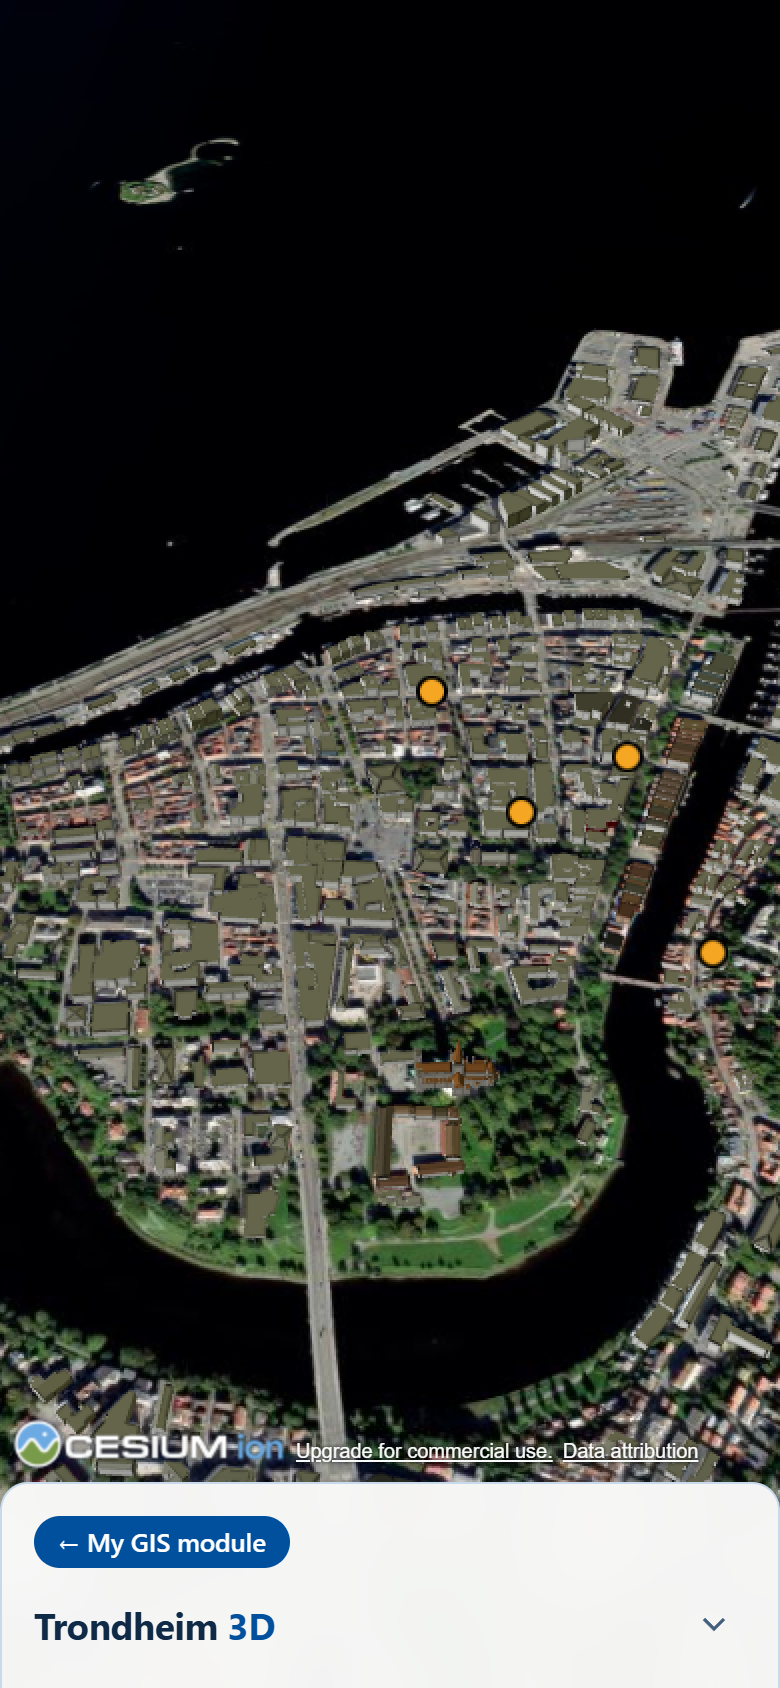
\includegraphics[width=\linewidth]{project-2-04-mobile.png}\caption{Trondheim 3D}\end{subfigure}\hfill
\begin{subfigure}{0.24\textwidth}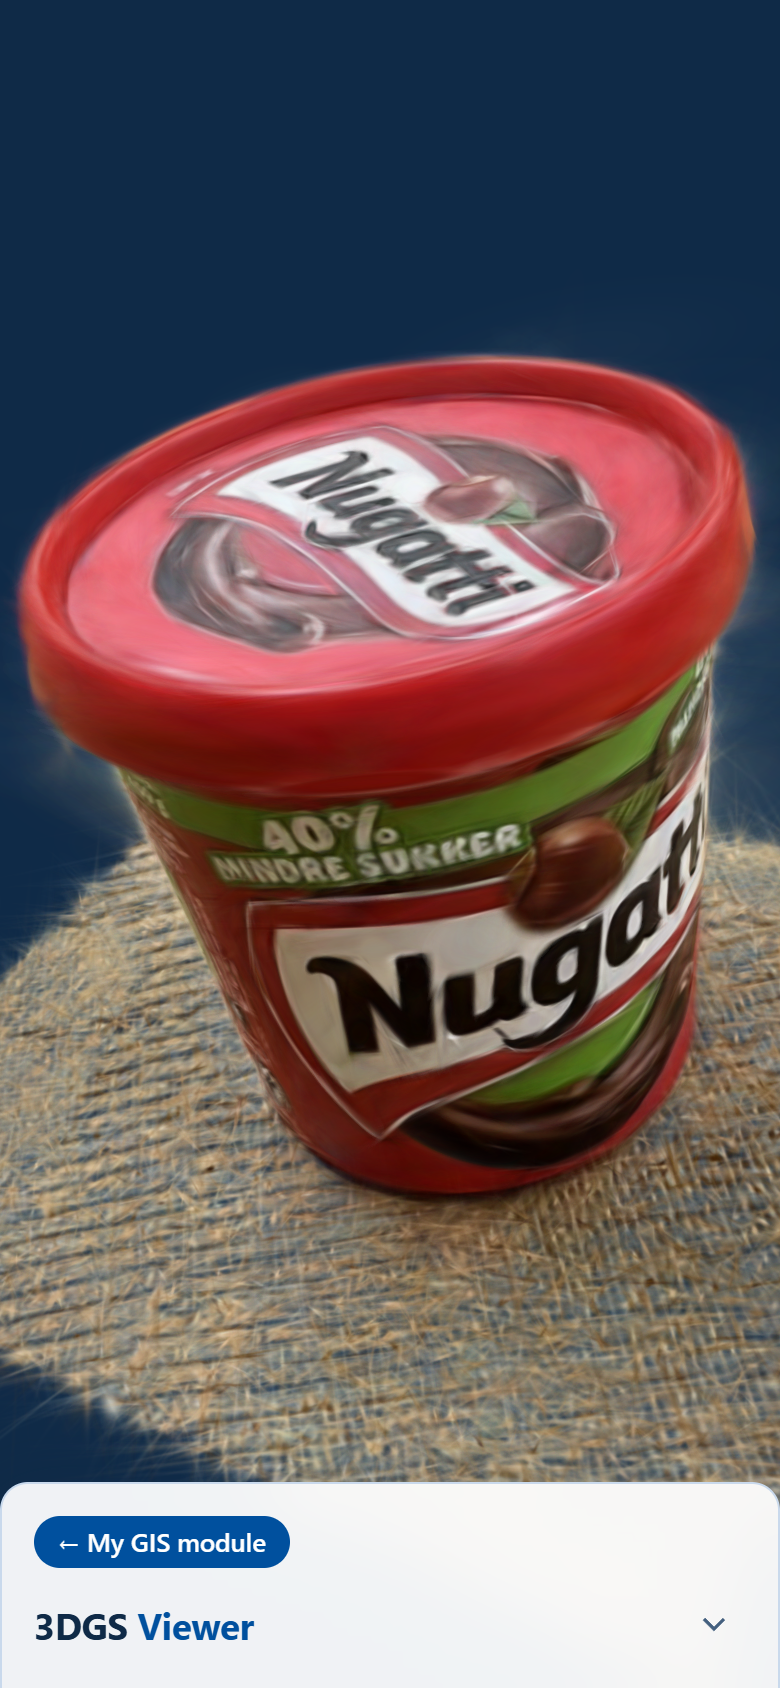
\includegraphics[width=\linewidth]{project-3-05-mobile.png}\caption{3DGS Viewer}\end{subfigure}
\caption{The site at phone width (390\,px). Each app links back to the homepage. Data: Natural Earth; \textcopyright{} OpenStreetMap contributors (ODbL); \textcopyright{} DSB (NLOD 2.0); Cesium ion.}
\label{fig:mobile}
\end{figure}

\section{Discussion}\label{sec:discussion}

% TODO (author): expand this reflection in your own words.
The three projects cover the three themes of the course from different angles. Projection Lab is GI science: a theoretical result ($\sec^2\varphi$ and Jensen's inequality) tested against measurement. Trondheim 3D is GI systems: most of its value lies in combining reference systems, data sources and services, and its analysis shows that a straight-line answer points to the wrong shelter at about one location in five. The 3DGS Viewer shows how far a popular new 3D data type still is from GIS use: without georeferencing it has no CRS, no reliable up direction and no scale.

Working with an AI coding assistant made the projects larger than I could have built alone, but it moved the work from writing code to directing and checking it. The most useful habits were to write the rules down (no invented numbers, verify before claiming), to require a runnable check for every change, and to inspect the screenshots myself. The pivot of the 3DGS project also showed the value of checking data access and licences before building on a dataset.

\section{Conclusion}\label{sec:conclusion}

Mercator inflates the median country area by $1.21\times$ and Greenland by $16.54\times$, and $\sec^2\varphi$ at the centroid predicts the inflation within 1\,\% for 156 of 176 countries while never overestimating it. In central Trondheim, the nearest public shelter on foot differs from the nearest in a straight line at 19\,\% of reachable grid points, and the median walk is 1.34 times the straight line. A Gaussian splat file can be opened and inspected entirely in the browser, but it carries no reference system, up direction or scale. All three apps are tested, documented and live at \siteurl.

\appendix
\section{Reproducing the results}\label{app:repro}

From the repository root (Windows PowerShell, Node 24, Python 3.14 with uv): \code{uv run --locked --project "Project 1/backend" pytest}; \code{npm --prefix "Project 2" test} and \code{npm --prefix "Project 3" test} (plus \code{run lint} and \code{run build}); the whole website with \code{npm run site:install} and \code{npm run site:build}. The Projection Lab database stack is described in \code{Project 1/README.md}.

\section{Data credits and licences}\label{app:credits}

Country boundaries: Natural Earth (public domain). Buildings and walking network: \textcopyright{} OpenStreetMap contributors (ODbL). Public shelters: \textcopyright{} DSB (NLOD 2.0). Terrain, imagery and 3D Tiles streaming: Cesium ion. Camera-target heights: Kartverket (CC BY 4.0). SOAR Telescope splat: Luis Cerda (CC BY 4.0). Splat rendering: Spark and three.js (MIT).
